Dette afsnit bygger på \cite{sandsynlighedsBog} og \cite{grimsandsynlighedsBog}.
\section{Loven om store tal}
\begin{theorem} \label{thm:Markovsulighed}[Markovs ulighed]
Hvis $X$ er en stokastisk variable, således
$E[X] < \infty$. Så gælder
\begin{align*}
    P(|X|\geq a) \leq \frac{E[|X|]}{a} \text{ for alle } a > 0
\end{align*}
\end{theorem}
\begin{proof}
Lad $A=\{|X|\geq a\}$, så fremstilles indikator funktionen af $A$, som $I_A$. Så tages den forventede værdi på begge sider, hvorefter man kan flytte $a$ uden for.
\begin{align*}
E[|X|]\geq E[aI_A] = a E[I_A] \iff \frac{E[|X|]}{a}\geq E[I_A]
\end{align*} 
hvor vi har benyttet at $E[I_A] = P(A)$. 
\end{proof}
Det er værd at bemærke, at hvis $a<0$ så skal relationen vendes om.

Chebyshews ulighed siger noget om, hvad sandsynligheden er for, at en stokastisk variabel ligger inden for $c$ gange standardafvigelser for middelværdien.
\begin{theorem} \label{Thm:Chebyshewsulighed}[Chebyshews ulighed]
    Lad $X$ være en stokastisk variable med middelværdien $\mu$ og variansen $\sigma^2>0$. For alle $c>0$ gælder, at 
    \begin{align*}
        P(|X-\mu|\geq c \sigma)\leq \frac{1}{c^2}
    \end{align*} 
\end{theorem}
\begin{proof}%fra wiki
    \begin{align*}
        P(|X-\mu|\geq c \sigma)=P((X-\mu)^2\geq c^2\sigma^2)
    \end{align*}
Ved at benytte Markovs ulighed, sætning \ref{thm:Markovsulighed} opnåes
\begin{align*}
    P((X-\mu)^2\geq c^2\sigma^2) \leq \frac{E[(X-\mu)^2]}{c^2\sigma^2}
\end{align*}
Da $E[(X-\mu)^2]$ er defineret af $\sigma^2$, så indsættes dette
\begin{align*}
    \frac{E[(X-\mu)^2]}{c^2\sigma^2} = \frac{\sigma^2}{c^2\sigma^2} = \frac{1}{c^2}
\end{align*}
Hvilket afslutter beviset.
\end{proof}

Loven om store tal beskriver, at ved en test med et stort antal forsøg vil den emperiske middelværdi, nærme sig den teoretiske middelværdi, jo flere forsøg der bliver foretaget.
\begin{thm} \label{thm:law_of_large_numbers}%theorem 4.1
    Lad $X_1, X_2, \dots$ være en følge af iid. med stokastisk variabler, med middelværdien $\mu$, of lad $\Bar{X}$ være den emperiske middelværdi. For hver $\varepsilon>0$ gælder at
    \begin{align*}
        P(|\Bar{X}-\mu|>\varepsilon) \rightarrow 0 \text{ når } n \rightarrow \infty
    \end{align*}
\end{thm}
\begin{proof}
    Antag at $X_k$ har en afgrænset varians, dvs $\sigma^2<\infty$. Anvend Chebyshews ulighed sætning \ref{Thm:Chebyshewsulighed}ulighed på $\Bar{X}$, og lad $c=\varepsilon \sqrt{x}/\sigma$. Eftersom $E[\Bar{X}]=\mu$ og $\Var[\Bar{X}]=\sigma^2/n$, dermed giver det
    \begin{align*}
        P(|\Bar{X}-\mu| > \varepsilon) \leq \frac{\sigma}{n\varepsilon^2} \rightarrow 0 \text{ når } n \rightarrow \infty
    \end{align*}
\end{proof}

\section{Simulering af diskrete variable} 
Vi vil i følgende afsnit antage at vi har en stokastisk variabel $U \sim \unif[0,1]$\footnote{Vi vil ikke gå mere i dybden vedrørende simulering af kontinuerte uniforme variable}, som vi vil benytte til at simulere diskrete variable, givet deres pmf.
\begin{thm} \label{thm:simuleringAfDiskreteVaraible}
    Lad $p$ være en pmf over det diskrete udfaldsrum $\{x_1, x_2, \ldots\}$, lad $F_0 = 0$ og
    \begin{equation*}
        F_n = \sum^n_{k = 1} p(x_k), \text{ for } n \in \N.
    \end{equation*}
    Lad $U \sim \unif[0, 1]$, og definer $X = x_n$ hvis $F_{n - 1} < U \leq F_n$, så har $X$ pmf $p$.
\end{thm}

\begin{proof}
    Da $U \sim \unif[0, 1]$ samt $X = x_n$ hvis og kun hvis $F_{n - 1} < U \leq F_n$ er
    \begin{equation*}
        P(X = x_n) = P(F_{n - 1} < U \leq F_n) = F_n - F_{n - 1} = p(x_n)
    \end{equation*}
    fordi $P(F_{n - 1} < U \leq F_n) = P\left(U \leq (F_n - F_{n - 1})\right)$.
\end{proof}

\begin{rem}
Hvis $p$ har tilhørende cdf $F$, så gælder det at $F_n = F(x_n)$ for $n \geq 1$.
\end{rem}
Følgende algoritme følger af sætning \ref{thm:simuleringAfDiskreteVaraible}, og gør det muligt at simulere diskrete fordelinger, givet den ønskede pmf $p$ og en uniform stokastisk variabel $U$ på intervallet $[0, 1]$.

\begin{algorithm} 
\caption{Simulering af diskrete fordelinger}\label{alg:discreteSimulation} 
\begin{algorithmic}[1] 
\Procedure{Discrete Distrubution} {$p: \{x_1, x_2, \ldots\} \rightarrow [0, 1]$, $U \sim \unif[0, 1]$}
 %$p$ er pmf'en for variablen som ønskes simuleret.
    \State $S := 0$
    \For{$k \in N$}
        \State $S' := S + p(x_k)$ 
        \If{$S < U \leq S'$} \Return $x_k$
        \EndIf
        \State $S := S'$
    \EndFor
\EndProcedure
\end{algorithmic}
\end{algorithm} 



\begin{exmp} \label{exmp:simuleringAfDiskreteVariable}
    Det ønskes at simulere $X \sim \Poi(1)$. Så har $X$ pmf $p(k) = \dfrac{\e^{-1}}{k!}$ for $k \in \N_0$.
    
    Algoritme \ref{alg:discreteSimulation} implementeres i appendix \ref{app:kodeTilSimuleringAfDiskreteVariable}. Her simuleres $n$ stokastiske variable som følger Poisson fordelingen og måler samtidig frekvensen $F_k$ af hvert udfald i udfaldsrummet $\N_0$.
    Af sætning \ref{thm:law_of_large_numbers} om store tal, kan vi approximere $p(k)$ som $\frac{F_k}{n}$ for $k = 0, 1, \ldots$, det benytter vi herefter til at lave følgende plot. 
    \begin{figure}[H]
        \centering
        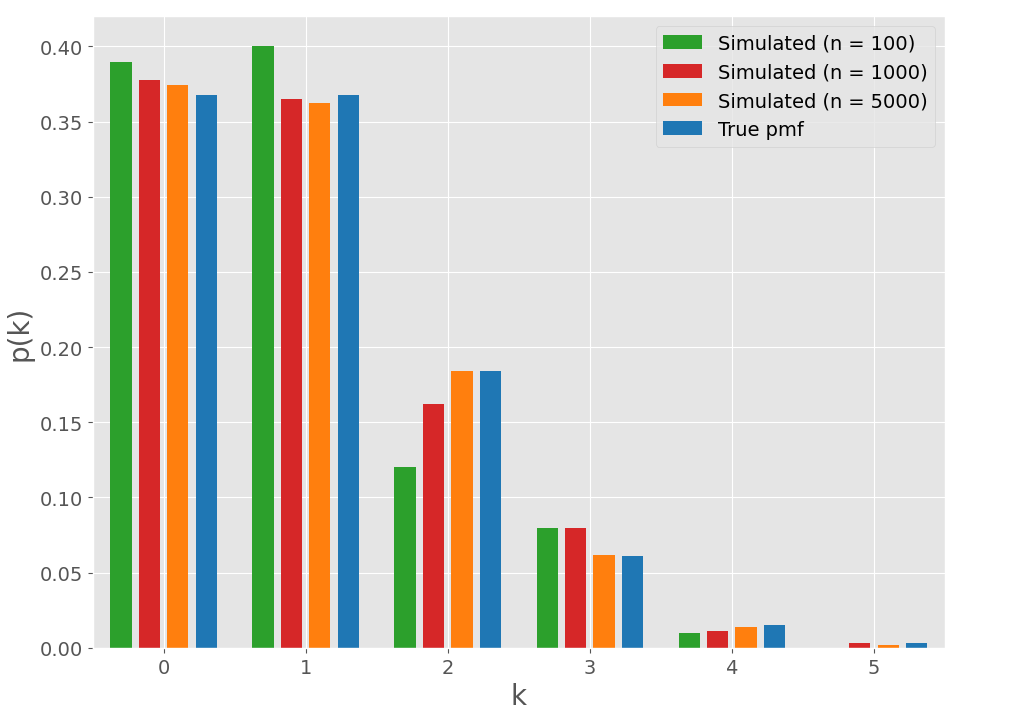
\includegraphics[scale=0.5]{fig/img/poisson.png} 
        \caption{Den simulerede relative frekvens af $k = 0, 1, \ldots, 5$ og den rigtige pmf.}
        \label{fig:simuleringAfPoisson}
    \end{figure}
    Det ses, at den simulerede relative frekvens af $k$ går imod $p(k)$, når $n$ vokser.
\end{exmp}

